\section{Phenomenology of On-Policy Distillation}
\label{sec:phenomenology}

Before investigating the token-level mechanism of OPD, we first ask a broader question: what conditions govern the effectiveness of OPD?
A natural assumption is that a stronger teacher should always yield better distillation outcomes, yet we observe configurations where this fails.
We compare OPD runs under controlled settings and identify two conditions that jointly govern the outcome.


\begin{tcolorbox}[takeawaysbox]
\begin{itemize}[topsep=0pt, partopsep=0pt, leftmargin=12pt, itemsep=0pt]
    \item \textbf{Thinking-pattern consistency.} The student and teacher should share compatible thinking patterns. Even when the teacher achieves higher benchmark scores, a large mismatch weakens the token-level distillation signal (\Cref{sec:thinking_pattern_consistency}).
    \item \textbf{Higher scores $\neq$ new knowledge.} The teacher should provide knowledge beyond what the student has seen during training. Even with consistent thinking patterns and higher scores, a teacher may offer no genuinely new knowledge, leaving OPD without a driving signal (\Cref{sec:information_gain}).
\end{itemize}
\end{tcolorbox}


\subsection{Thinking-Pattern Consistency}
\label{sec:thinking_pattern_consistency}

\begin{figure*}[t]
    \centering
    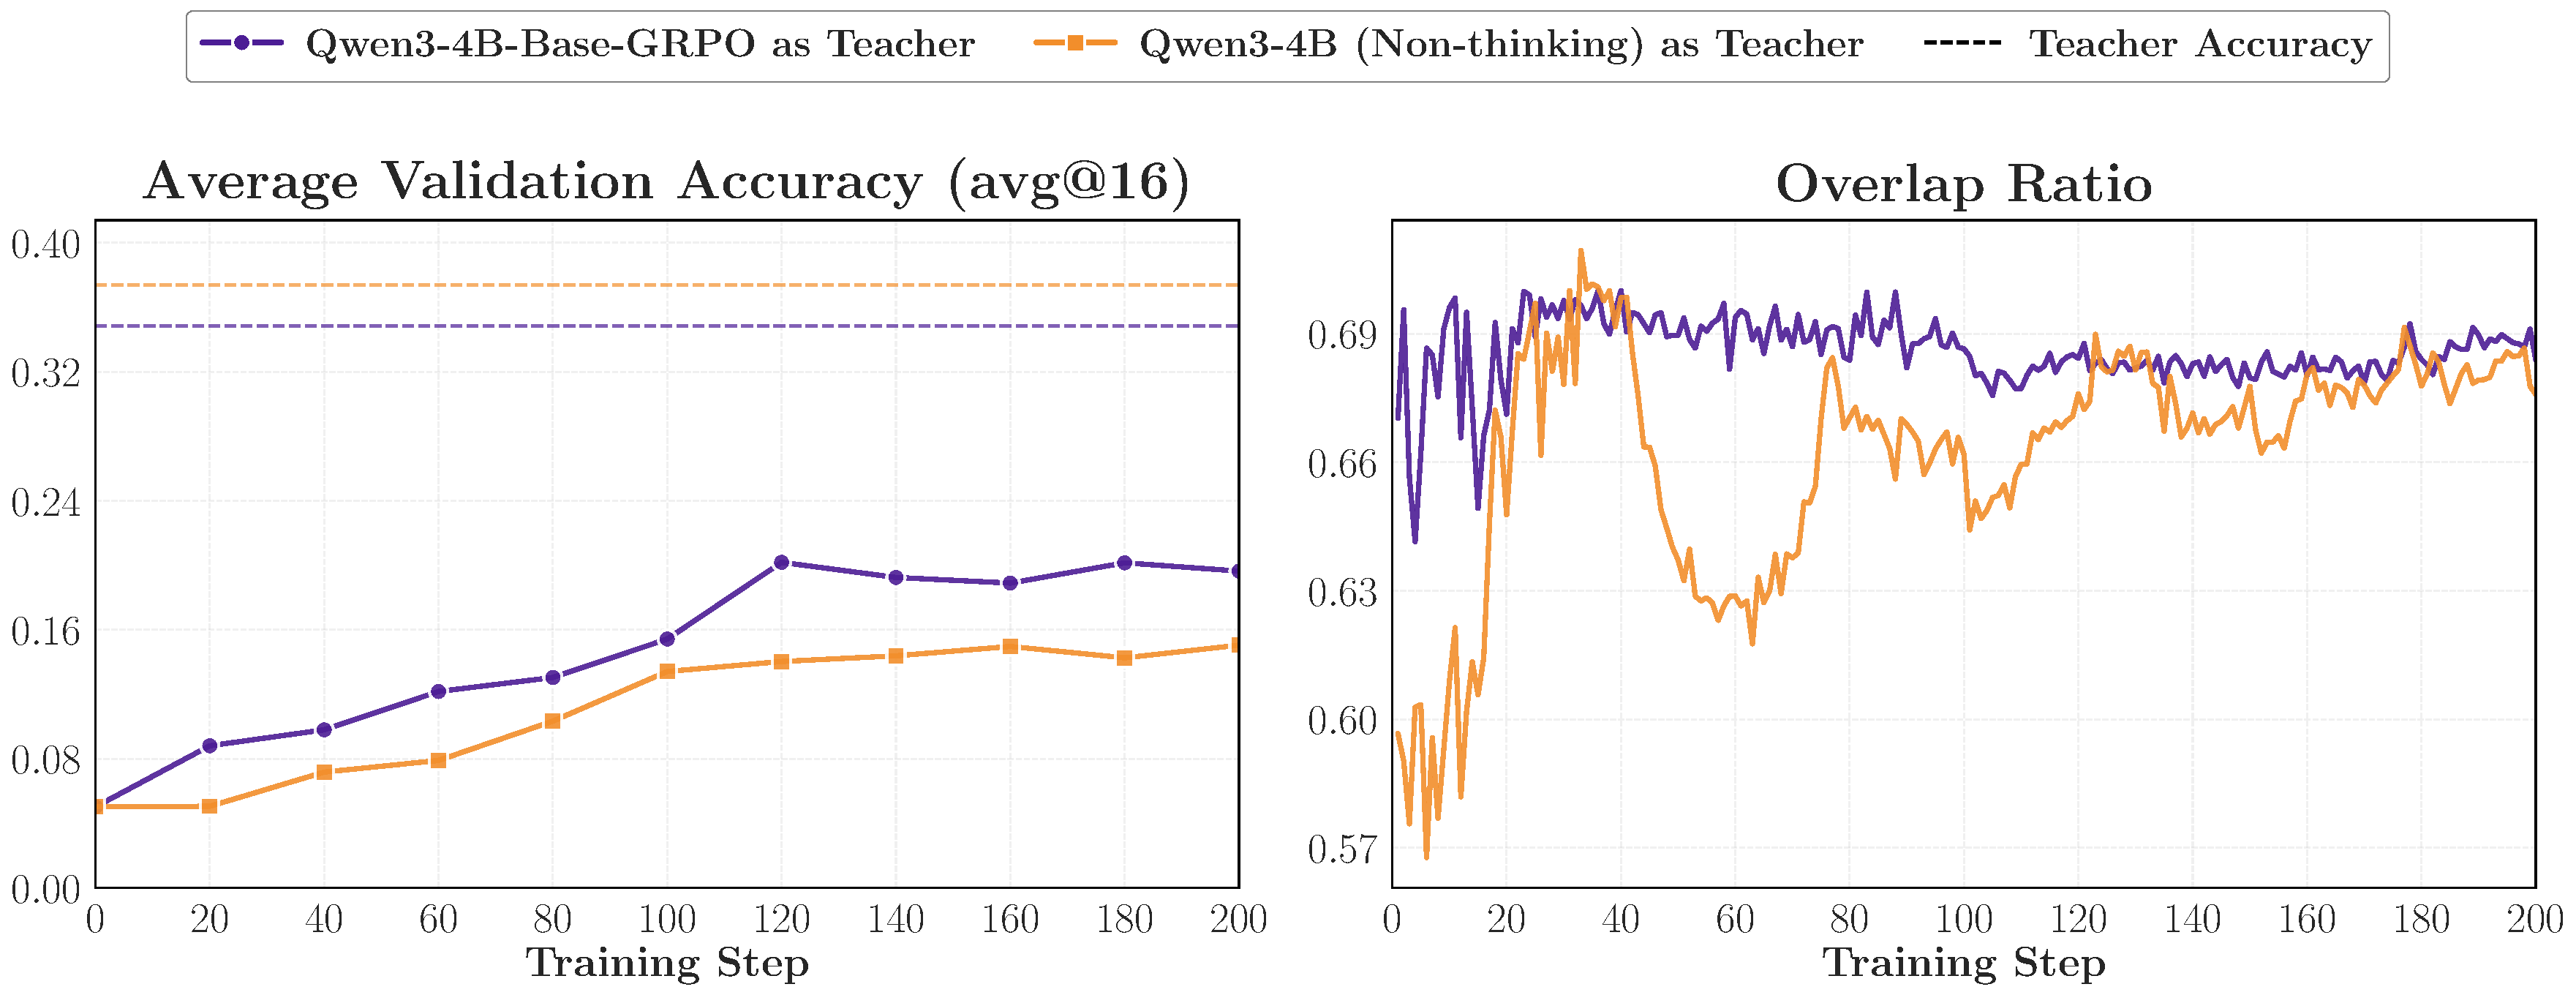
\includegraphics[width=\textwidth]{Figures/3.1/3_1_metrics.pdf}
    \caption{
    OPD from two teachers with different thinking patterns into the same student (Qwen3-1.7B-Base). The GRPO teacher achieves stronger performance (left) and higher initial overlap ratio (right), suggesting that thinking pattern compatibility governs OPD effectiveness.
    }
    \label{fig:thinking_pattern_compatibility}
\end{figure*}

We first study whether OPD requires compatible thinking patterns between the student and the teacher. A stronger teacher does not guarantee better distillation: a large mismatch in reasoning pattern can weaken the distillation signal regardless of the teacher's benchmark advantage.


\paragraph{Setup.}
We use Qwen3-1.7B-Base~\citep{yang2025qwen3} as the student and compare two teachers: Qwen3-4B (Non-thinking)~\citep{yang2025qwen3} and Qwen3-4B-Base-GRPO, where the latter is obtained by applying zero-RL to Qwen3-4B-Base~\citep{yang2025qwen3} using GRPO~\citep{shao2024deepseekmath} (detailed training settings are provided in Appendix~\ref{app:grpo_details}).
Since the student is also a base model, we expect its thinking pattern to be closer to that of the GRPO-trained teacher. We conduct two OPD experiments using the DAPO-Math-17K dataset~\citep{yu2025dapo}, differing only in the choice of teacher model. Unless otherwise specified, all experiments use the default hyperparameters described in Appendix~\ref{app:experimental_setup} and are evaluated on AIME 2024~\citep{li2024numinamath}, AIME 2025~\citep{balunovic2025matharena} and AMC 2023~\citep{li2024numinamath}.
Following standard practice, we sample 16 solutions per problem with temperature 0.7 and top-$p$ 0.95, using a maximum validation response length of 31{,}744 tokens. We report average accuracy over 16 samples (avg@16) as the primary evaluation metric.


\begin{wrapfigure}{r}{0.5\textwidth}
    \centering
    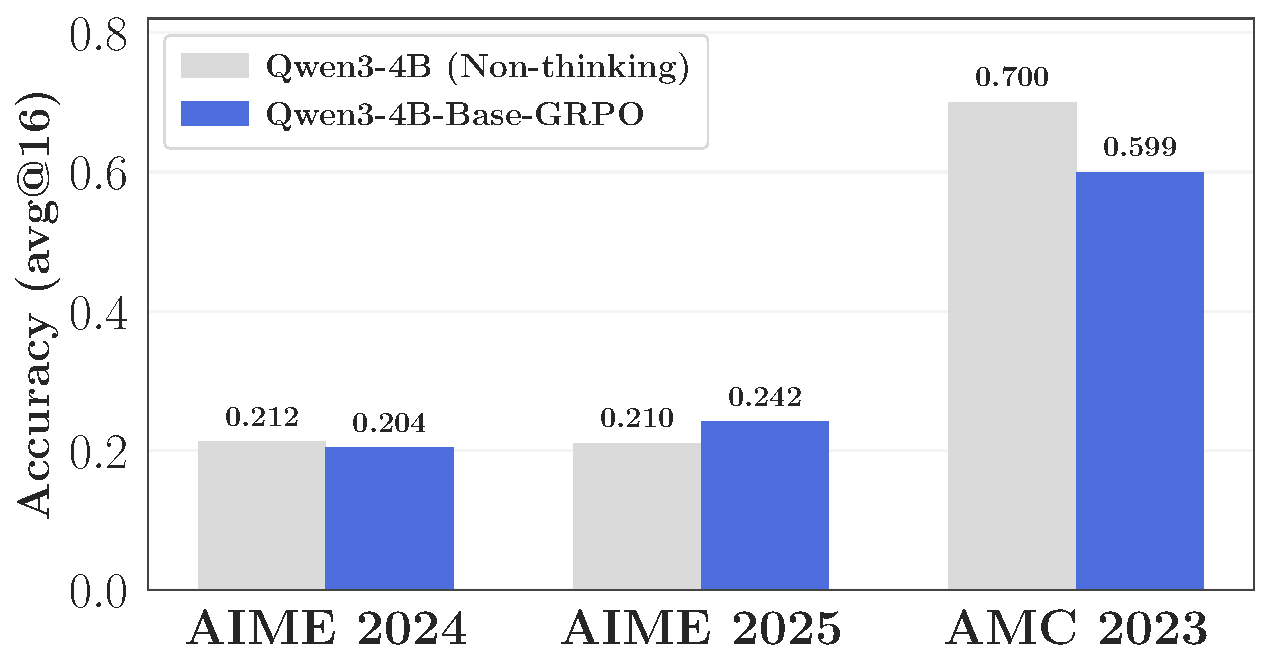
\includegraphics[width=\linewidth]{Figures/4.1/tch_val/5_1_teacher_perf.pdf}
    \caption{Validation performance of the two teachers (Qwen3-4B Non-thinking vs.\ Qwen3-4B-Base-GRPO) on AIME 2024, AIME 2025, and AMC 2023.
    }
    \label{fig:thinking_pattern_teacher_perf}
\end{wrapfigure}


\paragraph{Results.}
As shown in \Cref{fig:thinking_pattern_compatibility}, distillation from Qwen3-4B-Base-GRPO consistently outperforms distillation from Qwen3-4B (Non-thinking), although the two teachers have broadly comparable performance as shown in \Cref{fig:thinking_pattern_teacher_perf}. 
Despite underperforming on benchmarks, the GRPO teacher exhibits a higher initial overlap ratio, suggesting that its thinking pattern aligns more closely with the student.
Although the two overlap curves converge later in training, the performance gap persists, suggesting that early-stage thinking-pattern mismatch causes a loss of distillation benefit that cannot be recovered later.
We report the validation accuracy for each benchmark individually in Appendix~\ref{app:thinking_pattern_breakdown}, where the same overall trend holds across all datasets.





\subsection{New Knowledge, Not Just Scale}
\label{sec:information_gain}

Thinking-pattern consistency alone does not explain all of our observations. Even when the teacher scores higher and shares a consistent thinking pattern with the student, OPD can still fail.










\paragraph{Setup.}
We construct two controlled comparisons across model families.
In the DeepSeek family, we use DeepSeek-R1-Distill-Qwen-1.5B (R1-Distill-1.5B)~\citep{guo2025deepseek} as the student and compare two teachers: DeepSeek-R1-Distill-Qwen-7B (R1-Distill-7B)~\citep{guo2025deepseek} and Skywork-OR1-Math-7B~\citep{he2025skywork}, where the latter is obtained by applying RL post-training to R1-Distill-7B.
In the Qwen family, we use Qwen3-1.7B (Non-thinking)~\citep{yang2025qwen3} as the student and compare two teachers: Qwen3-4B (Non-thinking) and Qwen3-4B-Non-Thinking-RL-Math~\citep{yang2026learning}, where the latter is obtained by applying RL to Qwen3-4B (Non-thinking) on a 57K subset of DeepMath~\citep{he2025deepmath}.
In both settings, the key contrast lies between a teacher from the same training pipeline and one that has acquired additional capabilities through further RL. All runs use the same dataset and training recipe as before.


\begin{figure*}[t]
    \centering
    \begin{minipage}[t]{0.49\textwidth}
        \vspace{0pt}
        \centering
        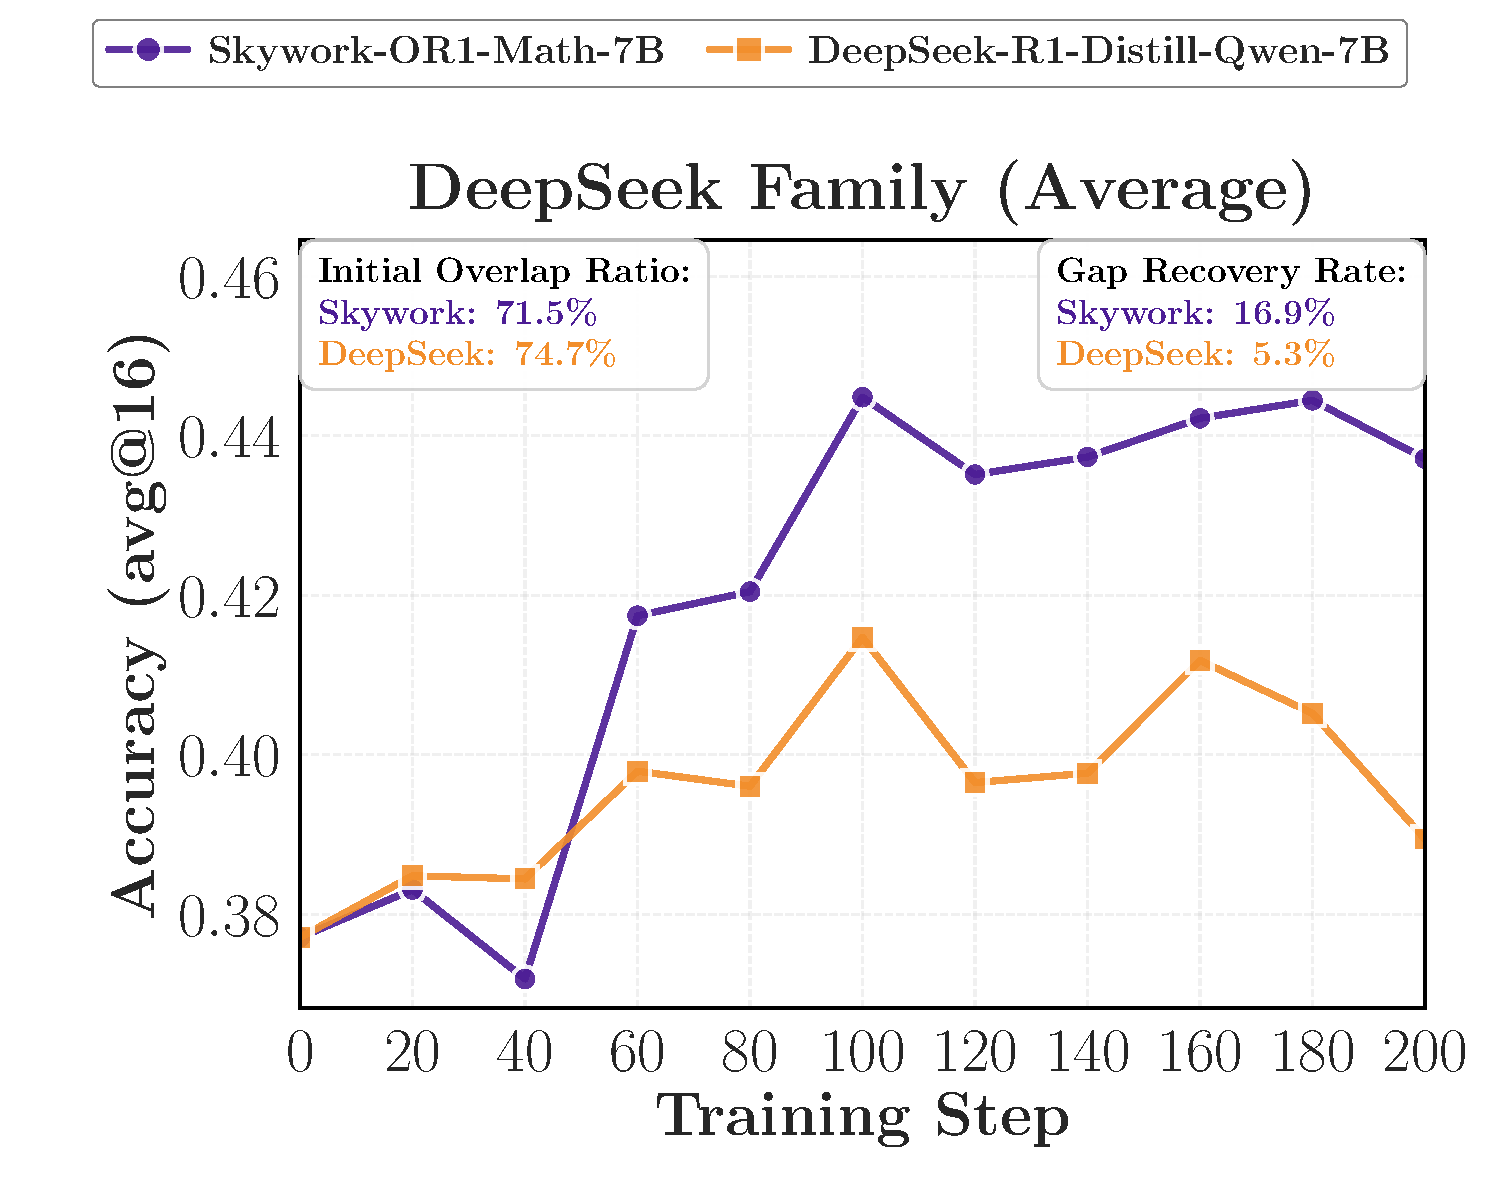
\includegraphics[width=\linewidth]{Figures/3.2/DS/Figure5A.pdf}
    \end{minipage}
    \hfill
    \begin{minipage}[t]{0.49\textwidth}
        \vspace{0pt}
        \centering
        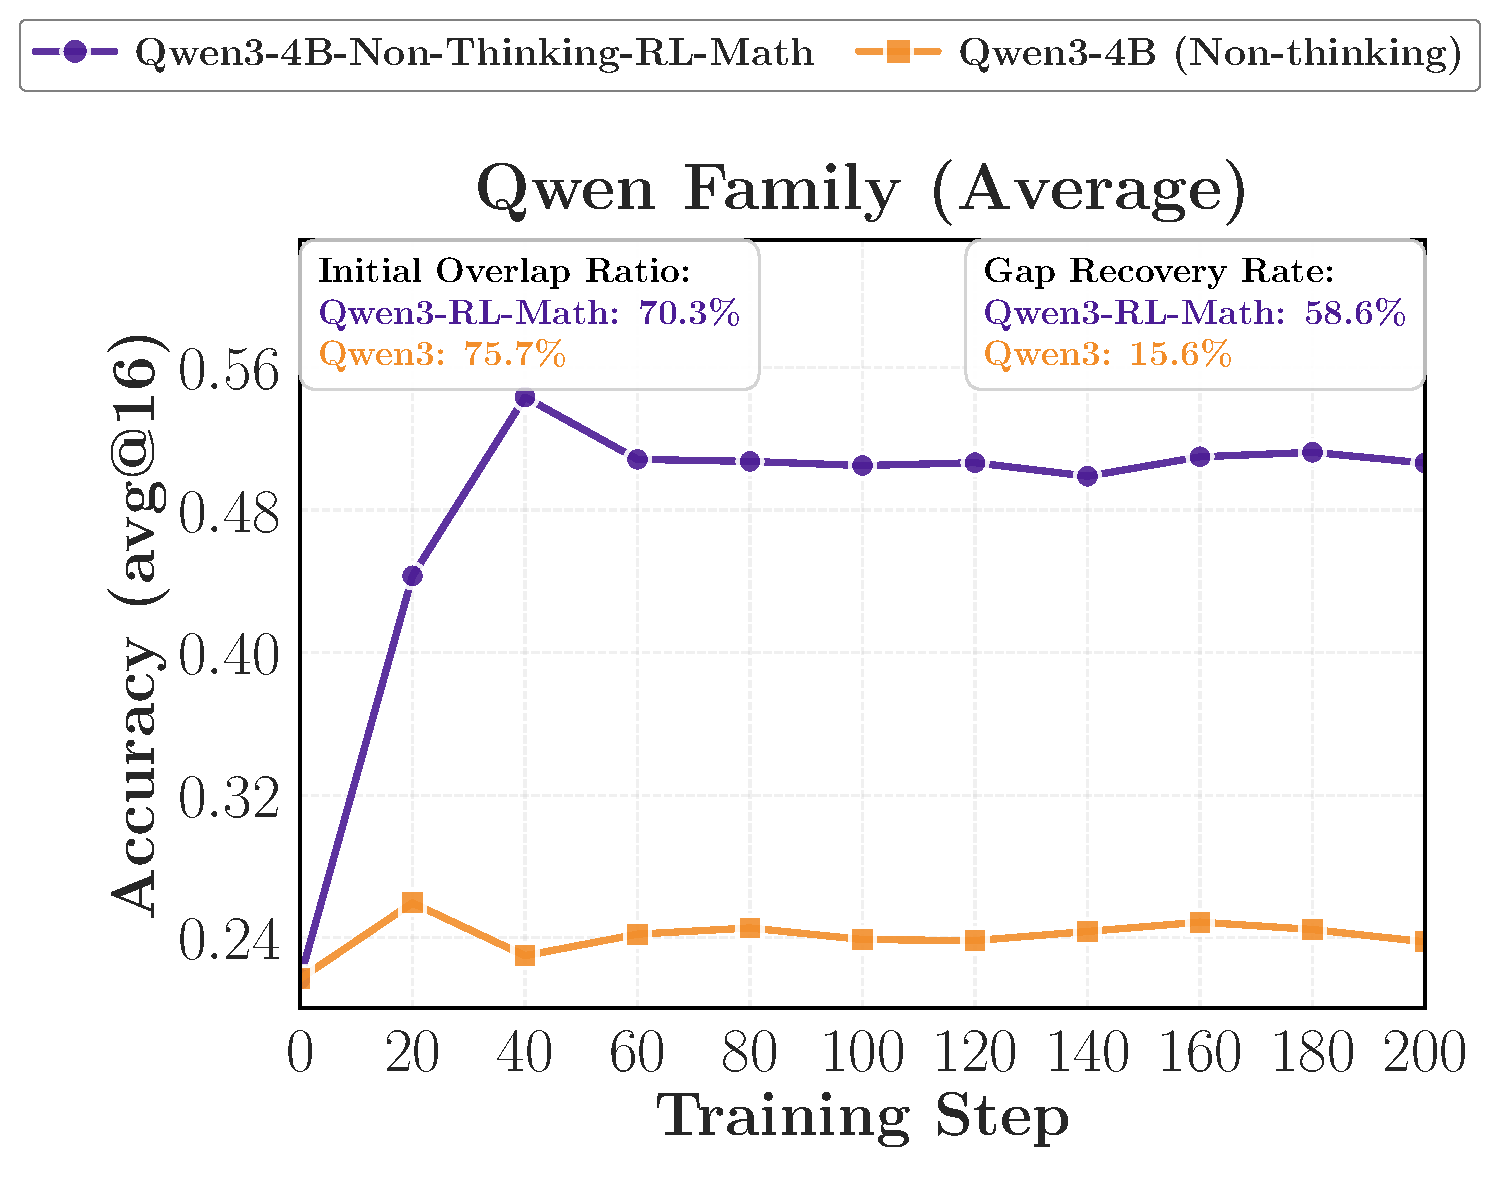
\includegraphics[width=\linewidth]{Figures/3.2/Qwen/Figure5B.pdf}
    \end{minipage}
    \caption{
    Comparison of OPD performance with and without additional teacher RL post-training across two model families.
    \textbf{Left:} DeepSeek family. \textbf{Right:} Qwen family.
    Post-trained teachers yield substantially stronger gains and higher teacher-student \emph{gap recovery rate}.
    }
    \label{fig:information_gain_main}
\end{figure*}


\paragraph{Results.}
As shown in \Cref{fig:information_gain_main}, both families exhibit a consistent pattern. \textbf{\textcolor[HTML]{F3983E}{Same-pipeline teachers}} yield limited improvement, while the \textbf{\textcolor[HTML]{4E1F96}{post-trained teachers}} produce substantially stronger gains across all benchmarks.
Importantly, the post-trained teachers not only achieve higher absolute performance but also recover a much larger fraction of the teacher-student gap, measured by the \emph{gap recovery rate} $(\mathrm{Acc}_{\text{after OPD}} - \mathrm{Acc}_{\text{before OPD}}) / (\mathrm{Acc}_{\text{teacher}} - \mathrm{Acc}_{\text{before OPD}})$.
This indicates that the additional capabilities acquired by these teachers are more transferable through OPD.
Since the post-trained teachers are derived from the same base checkpoints, their thinking patterns remain broadly aligned, which is also observed by the overlap ratio dynamic.
The improvement therefore stems from new capabilities of the teacher acquired through RL.






\subsection{Validation via Reverse Distillation}
\label{sec:reverse_distillation}

We design a reverse-distillation experiment as the comparison that simultaneously validates both conditions and reveals deeper insights into the nature of OPD.

\paragraph{Setup.}
JustRL-DeepSeek-1.5B (JustRL-1.5B)~\citep{he2025justrl} is obtained by RL from R1-Distill-1.5B. We now reverse this direction, using JustRL-1.5B as the student and distilling from R1-Distill-1.5B (its own pre-RL checkpoint).
We also use R1-Distill-7B as a teacher for the comparison.
Note that R1-Distill-7B achieves slightly higher benchmark scores than JustRL-1.5B, while R1-Distill-1.5B is substantially weaker.

\begin{figure*}[t]
    \centering
    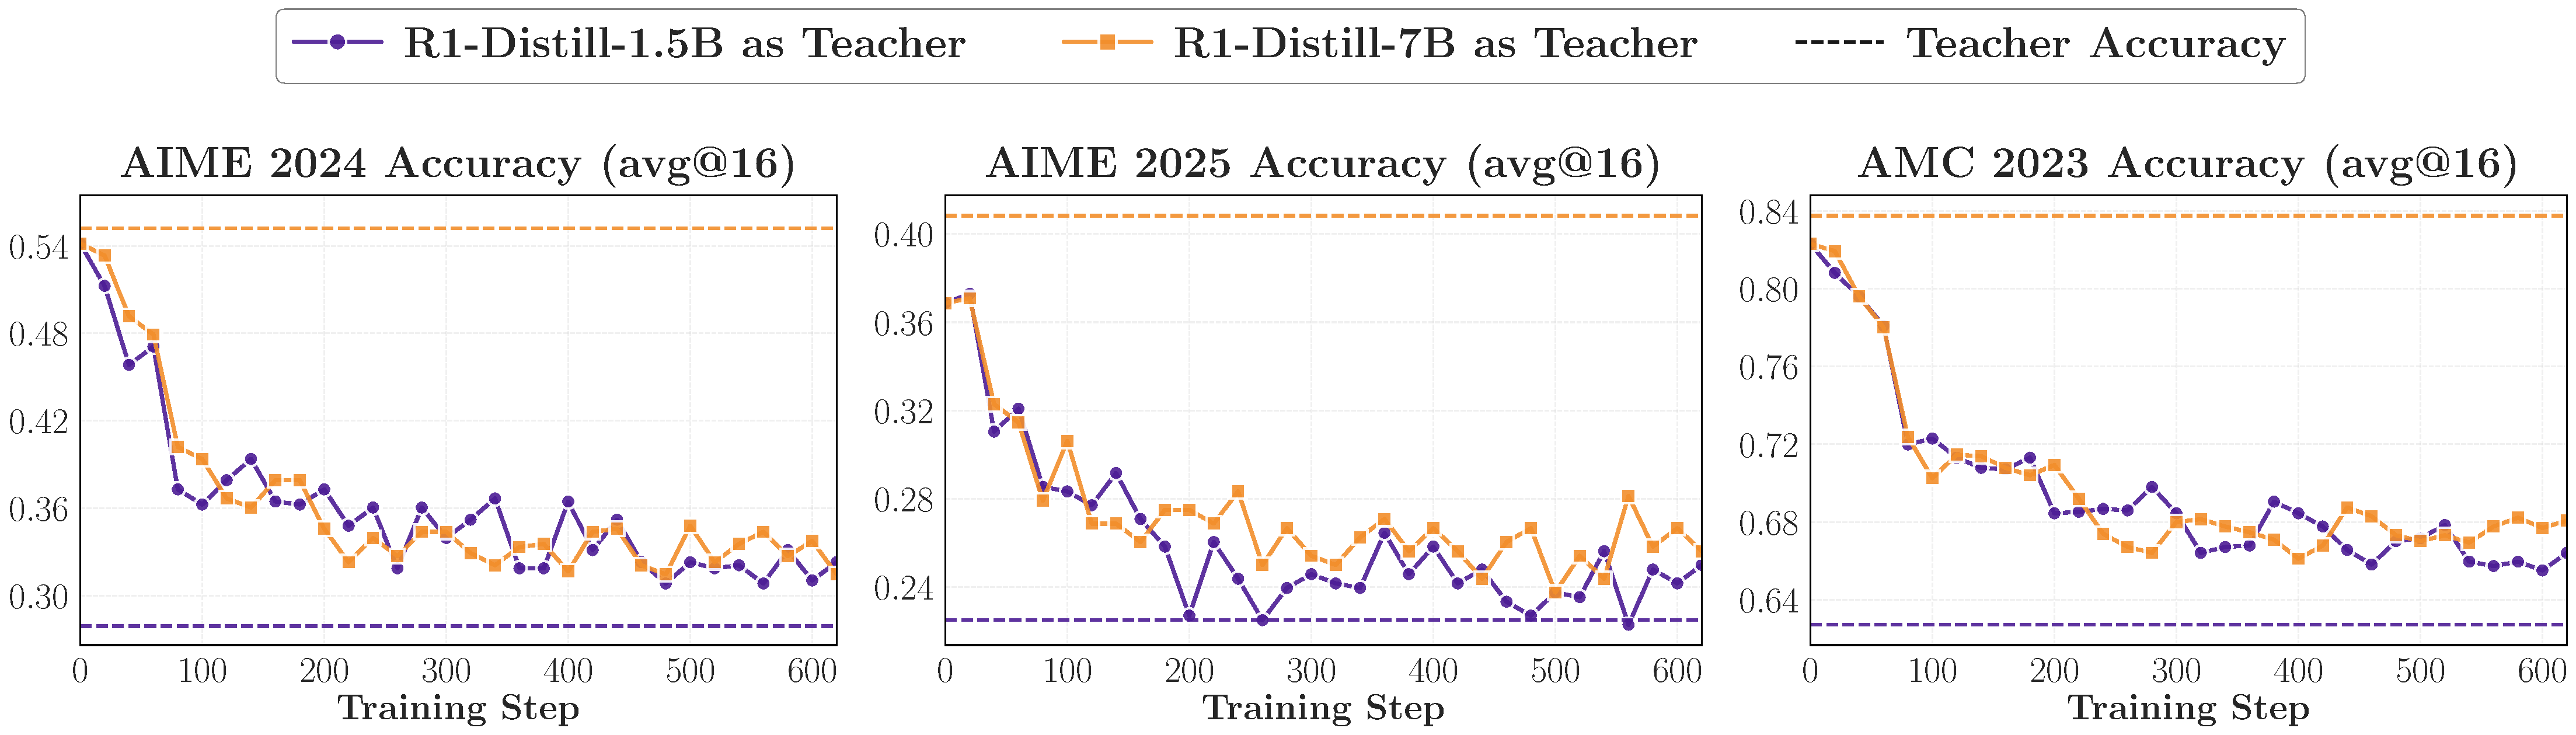
\includegraphics[width=\textwidth]{Figures/3.2/JustRL/JustRL_val.pdf}
    \caption{
    Reverse distillation with JustRL-1.5B as the student and two same-family teachers (R1-Distill-1.5B and R1-Distill-7B). Both runs cause the student to regress to approximately the same level despite R1-Distill-7B scoring higher than JustRL-1.5B, indicating that OPD training dynamics are governed by thinking pattern rather than benchmark performance.
    }
    \label{fig:information_gain_reverse}
\end{figure*}

\paragraph{Results.}
\Cref{fig:information_gain_reverse} reveals two striking phenomena.
First, distilling JustRL-1.5B toward R1-Distill-1.5B, its own pre-RL checkpoint, causes the student to regress almost exactly to its pre-RL performance, removing all gains acquired through RL.
Second, when we replace the teacher with R1-Distill-7B, a substantially larger and even slightly stronger model from the same family, the training trajectory is nearly indistinguishable: despite outscoring JustRL-1.5B on benchmarks, R1-Distill-7B drives the student to the same regressed level as the weaker 1.5B teacher.
Since OPD minimizes reverse KL divergence over student-generated trajectories, this convergence implies that the two teachers induce nearly identical local target distributions on student-visited states, despite their difference in scale.

These results yield several conclusions:
\begin{itemize}[leftmargin=12pt]
    \item \textbf{Thinking pattern matters, and OPD fundamentally learns thinking patterns.}
    Distilling from R1-Distill-1.5B into JustRL-1.5B causes JustRL-1.5B to regress to its pre-RL performance.
    This suggests that OPD actively acquires the teacher’s thinking patterns and overwrites the student's own. This is precisely why consistency in thinking patterns is important: if the gap is too large, the student may fail to learn effectively.
    
    \item \textbf{Benchmark performance does not predict OPD outcome.} R1-Distill-7B scores higher than JustRL-1.5B, yet the distillation produces no improvement and instead causes regression. This shows that OPD’s training dynamics can be completely independent of the teacher’s benchmark performance, and may even move in the opposite direction.
    
    \item \textbf{Higher scores do not imply new knowledge for OPD.} R1-Distill-7B and R1-Distill-1.5B are within the same model family and differ only in scale. The indistinguishable effects of the two models on the student already confirm that: (i) a higher score (R1-Distill-7B) may merely reflect a different degree of fit to the same data, rather than genuinely novel capabilities. For OPD to produce gains, the teacher should possess knowledge beyond what the student has already seen during training; and (ii) despite the difference in scale, R1-Distill-7B and 1.5B exhibit the same thinking patterns.

\end{itemize}


The reverse distillation experiments and the forward comparisons in \Cref{sec:thinking_pattern_consistency,sec:information_gain} consolidate the two conditions.
Thinking-pattern consistency is associated with higher initial overlap and stronger OPD outcomes, while new knowledge (such as from further post-training) enables larger transferable gains even when overlap is already high.
